% Search for all the places that say "PUT SOMETHING HERE".

\documentclass[11pt]{article}
\usepackage{amsmath,textcomp,amssymb,graphicx,enumerate,hyperref,enumitem,mathtools,tikz-qtree,listings,chemformula,bm,graphicx,grffile,gensymb,physics,amssymb,datetime,siunitx,multicol,pgfplots}
\graphicspath{{/Users/jonathansun5/Documents/Fall 2017/MCB 166/Homeworks/HW 6/Screen Shot 2017-11-29 at 11.42.43 PM.png} {/Users/jonathansun5/Documents/Fall 2017/MCB 166/Homeworks/HW 6/Screen Shot 2017-11-30 at 12.01.12 AM.png} {/Users/jonathansun5/Documents/Fall 2017/MCB 166/Homeworks/HW 6/Screen Shot 2017-11-30 at 12.08.22 AM.png} {/Users/jonathansun5/Documents/Fall 2017/MCB 166/Homeworks/HW 6/Screen Shot 2017-11-30 at 12.17.53 AM.png} {/Users/jonathansun5/Documents/Fall 2017/MCB 166/Homeworks/HW 6/Screen Shot 2017-11-30 at 10.28.34 AM.png}}
\pgfplotsset{compat=1.14}
\makeatletter
\newcommand{\leqnos}{\tagsleft@true\let\veqno\@@leqno}
\newcommand{\reqnos}{\tagsleft@false\let\veqno\@@eqno}
\reqnos
\makeatother

\def\Name{Jonathan Sun}  % Your name
\def\SID{25020651}  % Your student ID number
\def\Homework{6} % Number of Homework
\def\Session{Fall 2017}


\title{MCB166 --- \Session --- Problem Set \Homework}
\author{\Name, SID \SID}
\markboth{MCB166 --- \Session --- Problem Set \Homework --- \Name}{MCB166 --- \Session --- Problem Set \Homework --- \Name}
\pagestyle{myheadings}
\newdate{date}{30}{11}{2017}
\date{\displaydate{date}}

\def\endproofmark{$\Box$}
\newenvironment{proof}{\par{\bf Proof:}}{\endproofmark\smallskip}

\usepackage[margin=1in]{geometry}



\begin{document}
\maketitle

\newpage
\begin{enumerate}[label=\arabic*.]
\item
The traces shown in the figure below represent synaptic currents measured under voltage clamp. The given voltages are the holding potentials with respect to the resting potential.
\begin{center}
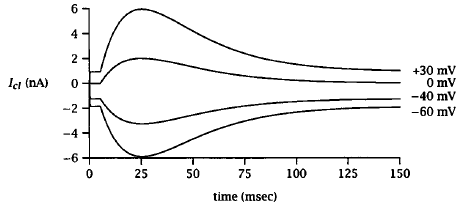
\includegraphics[width=0.75\textwidth]{/Users/jonathansun5/Documents/Fall 2017/MCB 166/Homeworks/HW 6/Screen Shot 2017-11-29 at 11.42.43 PM.png}
\end{center}
\begin{enumerate}[label=(\alph*)]
\item
What are the conductance and the reversal potential for this synaptic input?
\vspace*{1\baselineskip}
\\
Since $G_s$ is the slope of the line for $I_s$ vs. $V_m$, I will solve for the points this. When $V_m = -60 \text{mV}$, $I_s = -4 \text{nA}$ and when $V_m = 30 \text{mV}$, $I_s = 5 \text{nA}$. From these two points, the slope would be:
\begin{align*}
G_s = \frac{5 \text{nA} - (-4 \text{nA})} {30 \text{mV} - (-60 \text{mV})} = \frac{9 \text{nA}} {90 \text{mV})} = 10^{-7} \text{S} = 100 \text{nS}
\end{align*}
Furthermore, since $V_{rev}$ is the $V_m$-intercept of the $I_s$ vs. $V_m$ line, I can find the $V_{rev}$ when $I_s = 0$. Therefore, $V_{rev} = -20 \text{mV}$.



\item
Is the synapse likely to be excitatory or inhibitory?
\vspace*{1\baselineskip}
\\
The synapse is likely to be inhibitory.



\item
What is the approximate input resistance of the cell?
\vspace*{1\baselineskip}
\\
The approximate input resistance of the cell would be the result of the holding potential divided by the holding current. From the data, the approximate input resistance of holding potential at $30 \text{mV}$ and holding current at $1 \text{nS}$ gives $30000000 \Omega$ while the approximate input resistance of holding potential at $-60 \text{mV}$ and holding current at $-2 \text{nS}$ also gives $30000000 \Omega$. Therefore, the approximate input resistance of the cell is $30000000 \Omega$.



\item
What is the approximate decay time constant of the synaptic current?
\vspace*{1\baselineskip}
\\
Because the time constant is measured by the time it takes for the current to decrease from its peak to about $37\%$ of its peak, the time it takes for this is about $50$ msec because the peak was reached at $25$ msec and $37\%$ of its peak at $75$ msec.



\item
Is the decay time constant voltage dependent? Show the calculations that led to your answer.
\vspace*{1\baselineskip}
\\
No, the decay time constant is not voltage dependent because different voltages will take the same time to reach their current peaks. For example, they all reached their current peaks at the $25$ msec mark.



\item
If $V_{rev}$ is not equal to $E_s$, what does this tell you about this synapse?
\vspace*{1\baselineskip}
\\
If $V_{rev}$ is not equal to $E_s$, tht means the excitatory synapses in the CNS terminate on dendrites that are electrically remote from the cell body.
\end{enumerate}



\newpage
\item
You are voltage-clamping a neuromuscular junction at $-80 \text{mV}$ (perfect space clamp), and you measure the following end-plate currents in response to low-frequency nerve stimulation: (EPCs, in nA) $0.3$, $0.5$, $0.7$, $1.1$, $1.5$, $1.1$, $0.9$, $1.3$, $1.1$, $0.5$, $0.5$, $0.7$, $0.7$, $1.1$, $0.5$, $0.5$, $0.9$, $1.3$.
\begin{enumerate}[label=(\alph*)]
\item
If you assume that $E_s = 0 \text{mV}$, what is the approximate synaptic conductance?
\vspace*{1\baselineskip}
\\
To solve for the synaptic conductance, I will first solve for the mean EPC, which is $0.84 \text{nA}$.
With this, the approximate synaptic conductance is $\frac{0.84 \text{nA}} {-(-80 \text{mV})} = 1.05 \times 10 ^{-8} \text{S}$.



\item
Without any knowledge about miniature EPCs, what is the mean number of quanta released per stimulus?
\begin{align*}
CV = \frac{\sigma} {mean}
\end{align*}
To solve for the variance, $\sigma$, I will need to run the data through the function:
\begin{align*}
\sigma ^ 2 = \frac{\sum {((\text{current} - 0.84) ^ 2})} {18}
\end{align*}
This gives me the variance, $\sigma$, as $0.34$. Using this, I can solve for $CV$:
\begin{align*}
CV = \frac{0.34} {0.84} \approx 0.41
\end{align*}
To solve for the mean number of quanta released per stimulus, I can use $CV$:
\begin{align*}
m = \frac{1} {CV ^ 2} \approx 5.95
\end{align*}



\item
From your answer in (b), what is the predicted number of failures during a $1000$-stimulus experiment?
\begin{align*}
N_0 = N e^{-m} \approx 1000 e^{-5.95} \approx 2.6
\end{align*}
Since $N_0$ is about $2.6$, this rounds up to $3$ so I would predict between $2$ and $3$ failures.



\item
What are two reasons why you measure fewer failures than predicted from your calculation in (c)?
\vspace*{1\baselineskip}
\\
Two reasons why are that there is not enough data from experiments and that we should not have used the Poisson model.
\end{enumerate}



\newpage
\item
You have found that two putative neurotransmitters (X and Y) cause depolarization of isolated retinal horizontal cells and that both responses reverse at $0 \text{mV}$. You want to determine whether X and Y use the same or different ligand-gated channels. You obtain the following results. In voltage clamp at $V_{\text{rest}}$, a saturating concentration of X alone causes a $2 \text{nA}$ inward current, and a saturating concentration of Y alone also causes a $2 \text{nA}$ inward current. Also, $G_{\text{rest}} = 10 \text{nS}$ and $V_{\text{rest}} = -100 \text{mV}$. Assume that there is no desensitization and that the neuron is passive (no voltage-dependent conductances).
\begin{enumerate}[label=(\alph*)]
\item
If X and Y use the same channels, calculate the expected membrane potential (under current clamp) with X alone, with Y alone, and with X and Y together. Similarly, calculate the expected total current under voltage clamp at $V_{\text{rest}}$ when X and Y are applied together.
\vspace*{1\baselineskip}
\\
Solving for ${G_s}_{X, Y}$:
\begin{align*}
{{G_{s}}_{X, Y}} = \frac{2 \text{nA}} {100 \text{mV}} = 2 \times 10^{-7} \text{S} = 20 \text{nS}
\end{align*}
Solving for the expected membrane potential:
\begin{align*}
E_{sum} = \frac{G_s E_s + G_r E_r} {G_s + G_r}
\end{align*}
Since all the $E_s = 0$ for X alone, Y alone, and with X and Y together:
\begin{align*}
E_{sum} = \frac{G_r E_r} {G_s + G_r} = \frac{10 \text{nS} \times -100 \text{mV}} {20 \text{nS} + 10 \text{nS}} \approx -33.33 \text{mV}
\end{align*}
Therefore, the expected membrane potential with X alone, with Y alone, and with X and Y together is $-33.33 \text{mV}$. Furthermore, the expected total current when X and Y are applied together is $2 \text{nA}$.



\item
Repeat part (a) for the expected results if X and Y use different channels.
\vspace*{1\baselineskip}
\\
If X and Y use different channels, the expected membrane potential with X alone and with Y alone will still be $-33.33 \text{mV}$. Furthermore, the expected total current with X alone and Y alone is also still $2 \text{nA}$.
\\
On the other hand, solving for the expected membrane potential for X and Y together:
\begin{align*}
E_{sum} &= \frac{G_X E_X + G_Y E_Y + G_r E_r} {G_X + G_Y + G_r} \\
 &= \frac{20 \text{nS} \times 0 \text{mV} + 20 \text{nS} \times 0 \text{mV} + 10 \text{nS} \times -100 \text{mV}} {20 \text{nS} + 20 \text{nS} + 10 \text{nS}} \\
 &= -20 \text{mV}
\end{align*}
Therefore, the expected membrane potential with X and Y together is $-20 \text{mV}$. Furthermore, the expected total current when X and Y are applied together is now $2 \text{nA} + 2 \text{nA} = 4 \text{nA}$.
\end{enumerate}



\newpage
\item
For this problem, it is convenient to think about an equivalent circuit of the receptor cell that illustrates the action of stimulating light.
\begin{center}
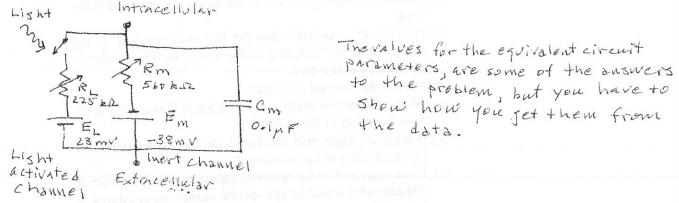
\includegraphics[width=0.75\textwidth]{/Users/jonathansun5/Documents/Fall 2017/MCB 166/Homeworks/HW 6/Screen Shot 2017-11-30 at 12.01.12 AM.png}
\end{center}
This problem concerns single visual cells in the ocellus of a barnacle (Brown, Hagiwara, Koike \& Meech, $1970$). Two glass microelectrods were inserted into the cell, one to record membrane potential and the other to pass inward or outward current pulses. At the same time a standard flash of light could be given (Fig. $13.5$).
\begin{center}
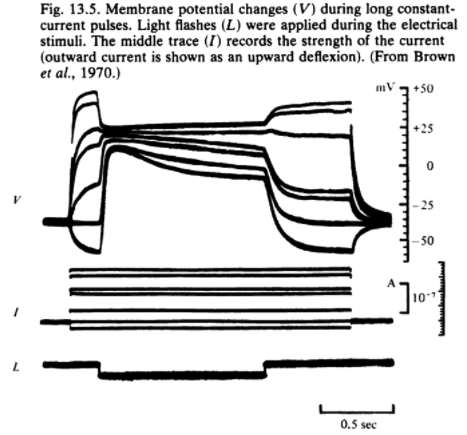
\includegraphics[width=0.75\textwidth]{/Users/jonathansun5/Documents/Fall 2017/MCB 166/Homeworks/HW 6/Screen Shot 2017-11-30 at 12.08.22 AM.png}
\end{center}
\begin{enumerate}[label=(\alph*)]
\item
Draw a text-figure graph of membrane potential against stimulus current, plotting curves for the receptor in the dark and after $0.5$ sec in the light during the flashes.
\begin{center}
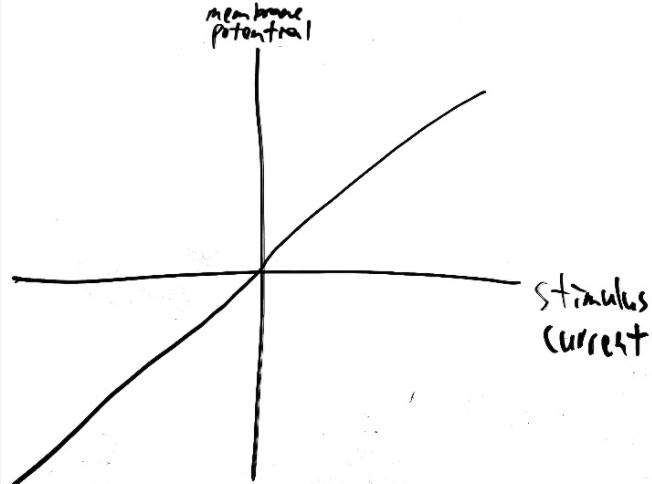
\includegraphics[width=0.75\textwidth]{/Users/jonathansun5/Documents/Fall 2017/MCB 166/Homeworks/HW 6/Screen Shot 2017-11-30 at 11.52.52 AM.png}
\end{center}



\item
What is the input resistance of the cell in the light and in the dark?
\vspace*{1\baselineskip}
\\
The input resistance of the cell in the light is $225 \text{k}\Omega$ and the input resistance of the cell in the dark is $560 \text{k}\Omega$.



\item
Give an approximate value for the time constant of the membrane in the dark, and deduce a value for the membrane capacitance in the dark.
\vspace*{1\baselineskip}
\\
Ok.



\item
What is the reversal potential?
\vspace*{1\baselineskip}
\\
It is the difference between $23 \text{mV}$ and $-38 \text{mV}$, which is $61 \text{mV}$.



\item
What conductance change for which ion or ions is most likely to be the effect of illumination?
\vspace*{1\baselineskip}
\\
Sodium ions are most likely to be the effect of illumination.



\item
Is there any clear evidence for (i) electrical excitability and (ii) rectification in the membrane?
\vspace*{1\baselineskip}
\\
Yes, since the sodium ions are most likely to be the effect of illumination so that suggests there is a electrogenic sodium pump.



\item
If you assume that the cells are spherical with a diameter of $100 \mu\text{m}$, what would be the specific membrane resistance in the dark?
\begin{align*}
\text{resistance} &= 560 \text{k}\Omega \times \text{surface area} \\
 &= 560 \text{k}\Omega \times 100 \mu\text{m} \\
 &= 180 \Omega \text{cm}^2
\end{align*}



\item
Microvilli are known to be present on the cells; how would this fact affect your estimate of specific membrane resistance?
\vspace*{1\baselineskip}
\\
The surface area would be larger, which will also make the specific membrane resistance larger as well.
\end{enumerate}



\newpage
\item
A neuron contains $N$ identical channels that are gated by the neurotransmitter glutamate. Glutamate opens these channels and results in an inward \ch{Na+} current ($E_{\ch{Na}} = +50 \text{mV}$). The glutamate-induced currents in this neuron under voltage-clamp conditions ($V_{\ch{P}} = 10 \text{mV}$) are given in the following diagram:
\begin{center}
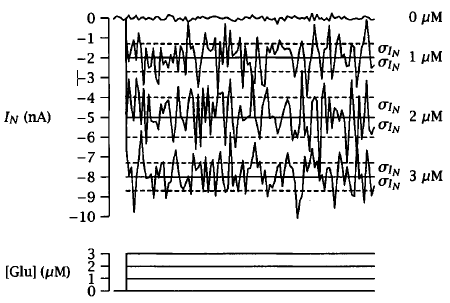
\includegraphics[width=0.75\textwidth]{/Users/jonathansun5/Documents/Fall 2017/MCB 166/Homeworks/HW 6/Screen Shot 2017-11-30 at 12.17.53 AM.png}
\end{center}
\begin{enumerate}[label=(\alph*)]
\item
Plot the variance (${{\sigma_{I}}_{N}}^2$) as a function of mean current $\mu_{I}$ on graph paper.
\vspace*{1\baselineskip}
\\
From the graph above, I am guestimating that ${\sigma_{I}}_{N} = \pm0.7 \text{nA}$ for $1 \mu\text{M}$ and $3 \mu\text{M}$ and ${\sigma_{I}}_{N} = \pm1 \text{nA}$ for $2 \mu\text{M}$. So, ${{\sigma_{I}}_{N}} ^ 2 = 1 \text{(nA)}^2$ for $2 \mu\text{M}$. Therefore, my graph is:
\begin{center}
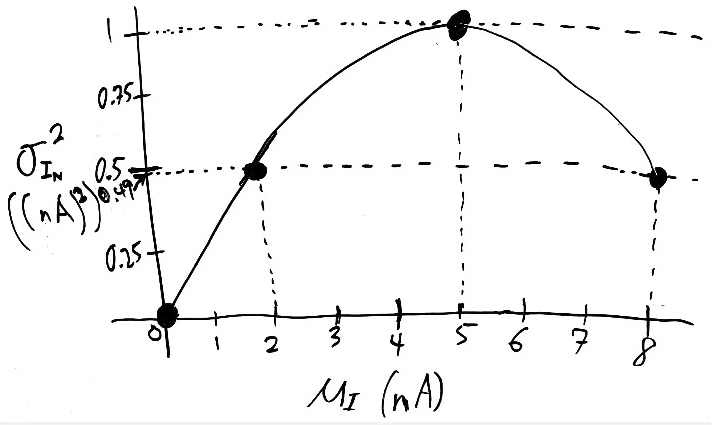
\includegraphics[width=0.75\textwidth]{/Users/jonathansun5/Documents/Fall 2017/MCB 166/Homeworks/HW 6/Screen Shot 2017-11-30 at 10.28.34 AM.png}
\end{center}



\item
Estimate the single-channel conductance and the total number of glutamate-gated channels in the neuron.
\begin{align*}
{{\sigma_{I}}_{N}} ^ 2 = I_1 \mu_I - \frac{{\mu_I}^2} {N}
\end{align*}
\begin{align*}
\frac{d} {d\mu_I} \left({{\sigma_{I}}_{N}} ^ 2\right) = \frac{d} {d\mu_I} \left(I_1 \mu_I - \frac{{\mu_I}^2} {N}\right) = I_1 - \frac{2 \mu_I} {N}
\end{align*}
When $\mu_I = 0$:
\begin{align*}
\frac{d} {d\mu_I} \left({{\sigma_{I}}_{N}} ^ 2\right) = I_1
\end{align*}
By definition, $\frac{d} {d\mu_I} \left({{\sigma_{I}}_{N}} ^ 2\right) = I_1$ is the slope of the curve at the origin. This slope is close to the slope between the origin and $1 \mu\text{M}$ and this slope is about:
\begin{align*}
\frac{0.49 \text{(nA)}^2} {2 \text{nA}} \approx \frac{0.5 \text{(nA)}^2} {2 \text{nA}} = 0.25 \text{nA} = I_1
\end{align*}
So, using this $I_1$:
\begin{align*}
\gamma = \frac{I_1} {V - E_i} = \frac{0.25 \text{nA}} {10 \text{mV} - 50 \text{mV}} = 6.25 \text{nS}
\end{align*}
From the graph, the maximum ${{\sigma_{I}}_{N}} ^ 2$ is at $\mu_I = 5 \text{nA}$. Using this to solve for the number of channels:
\begin{align*}
N = \frac{2 \mu_I^m} {I_1} \approx \frac{2 \times 5 \text{nA}} {0.25 \text{nA}} = 40
\end{align*}
Therefore, there is about 40 glutamate-gated channels in the neuron.
\end{enumerate}
\end{enumerate}
\end{document}
